\section*{Exercise 3}

\subsection*{Exercise 3.2}
Explain why (in terms of the evaluation process) these two programs give different answers 
(i.e. have different distributions on return values):
\begin{lstlisting}
(define foo (flip))
(list foo foo foo)
\end{lstlisting}

\begin{lstlisting}
(define (foo) (flip))
(list (foo) (foo) (foo))
\end{lstlisting}    

\paragraph{Solution} 
In the first program we are defining \texttt{foo} as a variable and we are assigning it the value of the evaluation of the 
expression \texttt{(flip)}, indeed, the value of \texttt{foo} is either \texttt{\#t} or \texttt{\#f}.
After that we create a list which contains three time the value of \texttt{foo}, so if \texttt{foo} has value \texttt{\#t}, then
we are defining a the list: \texttt{'(\#t \#t \#t)}; otherwise we are creating the list: \texttt{'(\#f \#f \#f)}.

In the second program, we are defining a new procedure \texttt{foo} which is a wrapper for the procedure \texttt{flip}. This means
that each time the procedure \texttt{foo} is called, also the procedure \texttt{flip} is called.
For this reason, when we define the list, the expression \texttt{flip} is evaluated three times and, since it is a non-deterministic 
procedure, the three elements of the list can be different.


\subsection*{Exercise 3.5}
Here is a modified version of the tug of war game. Instead of drawing strength from the continuous Gaussian 
distribution, strength is either 5 or 10 with equal probability. Also the probability of laziness is changed from 1/4 to 1/3. 
Here are four expressions you could evaluate using this modified model:

\begin{lstlisting}
(define strength (mem (lambda (person) (if (flip) 5 10))))
(define lazy (lambda (person) (flip (/ 1 3))))
    
(define (total-pulling team)
  (sum
   (map (lambda (person) (if (lazy person)
                             (/ (strength person) 2)
                             (strength person)))
        team)))
    
(define (winner team1 team2)
  (if (< (total-pulling team1) (total-pulling team2))
      team2
      team1))
    
(winner '(alice) '(bob))                        ;; expression 1
    
(equal? '(alice) (winner '(alice) '(bob)))      ;; expression 2
    
(and (equal? '(alice) (winner '(alice) '(bob))) ;; expression 3
     (equal? '(alice) (winner '(alice) '(fred))))
    
(and (equal? '(alice) (winner '(alice) '(bob))) ;; expression 4
     (equal? '(jane) (winner '(jane) '(fred))))
\end{lstlisting}

\begin{itemize}
    \item[a.] Write down the sequence of expression evaluations and random choices that will be made in evaluating each expression.
    \item[b.] Directly compute the probability for each possible return value from each expression.
    \item[c.] Why are the probabilities different for the last two? Explain both in terms of the probability calculations 
        you did and in terms of the “causal” process of evaluating and making random choices.
\end{itemize}

\paragraph{Solution}
\begin{itemize}
    \item[a.] First of all, the procedures are defined and the interpreter associates the name of the procedures with their definition
        in the \textit{global environment}.
        Then the interpreter evaluates the four expressions in the order in which they are written: 
        
        \paragraph*{Expression 1} \texttt{(winner '(alice) '(bob))} 
        
        The first step is to retrieve the body of the procedure \texttt{winner} and then the formal parameters are substituted by 
        the actual parameters \texttt{'(alice)} and \texttt{'(bob)}. 
        Now the interpreter has to evaluate the following expression:
        \begin{lstlisting}[caption={Body of procedure \texttt{winner} with actual parameters}, captionpos=b]
(if (< (total-pulling '(alice)) (total-pulling '(bob)))
    '(bob)
    '(alice)))  
        \end{lstlisting}
        The following step is to evaluate the conditional expression, so it starts by evaluating the \textit{predicate}: 
        \texttt{(< (total-pulling '(alice)) (total-pulling '(bob)))}. The interpreter has to deal with the primitive predicate
        \texttt{<}, so it needs to evaluate the arguments and than apply the predicate to the evaluated arguments.
        The first argument to evaluate is \texttt{(total-pulling '(alice))}: the body of the procedure \texttt{total-pulling} 
        is retrieved in the \textit{global environment} and it is substituted by the expression, 
        then the actual parameter is applied to the body of the procedure. The expression \texttt{(total-pulling '(alice))} becomes
        as follows:
        \begin{lstlisting}[caption={Body of procedure \texttt{total-pulling} with actual parameters}, captionpos=b, label={lst:t-p}]
(sum
 (map (lambda (person) (if (lazy person)
                           (/ (strength person) 2)
                           (strength person)))
      '(alice)))
        \end{lstlisting}
        The procedure \texttt{sum} takes as argument a list of numbers and returns the sum over the elements of the list. In this case
        the argument of the procedure is another expression, so the interpreter has to evaluate the argument and then apply it to the
        procedure \texttt{sum}.
        Now the expression to be evaluated is the following:
        \begin{lstlisting}[caption={Argument of procedure \texttt{sum} in Listing~\ref{lst:t-p}}, captionpos=b, label={lst:map}]
(map (lambda (person) (if (lazy person)
                          (/ (strength person) 2)
                          (strength person)))
     '(alice))
        \end{lstlisting}
        The procedure \texttt{map} takes as arguments a \textit{lambda} expression and a list. The procedure applies the
        \textit{lambda} expression to each element of the list and returns the list of the results of the \textit{lambda}
        expression on the elements of the list in input.
        So the first step is to evaluate the \textit{lambda} expression with argument \texttt{'alice}. The resulting expression is
        the body of the \textit{lambda} expression with actual parameter \texttt{'alice}:
        \begin{lstlisting}[caption={Application of \texttt{map} prcedure of Listing~\ref{lst:map}}, 
            captionpos=b, label={lst:lambda-body}]
(if (lazy 'alice) (/ (strength 'alice) 2) (strength 'alice))
        \end{lstlisting}
        Since the interpreter has to evaluate a conditional expression, the interpreter firsts evaluate the \textit{predicate}.
        To evaluate the call \texttt{(lazy 'alice)}, the interpreter first takes the body of the procedure and then substitutes
        all the occurences of formal parameter by the value of the actual parameter. The resulting expression is:
        \begin{lstlisting}[caption={Body of procedure \texttt{lazy} when evaluating Listing~\ref{lst:lambda-body}}, captionpos=b]
(flip (/ 1 3))
        \end{lstlisting}
        The procedure \texttt{flip} is a probabilistic procedure, it can take as parameter the probability to return \texttt{\#t}.
        In our case, the interpreter has to evaluate the expression \texttt{(/ 1 3)} and than apply the result to the procedure 
        \texttt{flip}.
        We suppose that the result of the call \texttt{(flip 1/3)} is \texttt{\#f}, so the result of the evaluation of the
        \textit{predicate} in the conditional expression is \texttt{\#f}. Since the \textit{predicate} is false, the interpreter has
        to evaluate the \textit{alternative} expression \texttt{(strength 'alice)}.
        It is a procedure call, so the interpreter has to retrieve the body of the procedure and then to substitute the formal
        parameter by the actual one.
        The result is that the interpreter now has to evaluate the following expression:
        \begin{lstlisting}[caption={Body of procedure \texttt{strength} when evaluating Listing~\ref{lst:lambda-body}}, captionpos=b]
(if (flip) 5 10)
        \end{lstlisting}
        The procedure \texttt{strength} is a particular type of procedure, indeed, it is memoized through the procedure \texttt{mem}.
        This means that the first time the procedure is called, the result of the call is memorized and each time the procedure is
        called with same the same argument, the interpreter does not evaluate the function, but it retireves the already computed
        result in the \textit{global environment}. This is the first time that \texttt{(strength 'alice)} is evaluated, 
        so the procedure has to be evaluated in a ``standard'' way.
        The body of the procedure is composed by a conditional expression, the procedure \texttt{flip} is evaluated and we suppose
        that the result is \texttt{\#t}, so the procedure \texttt{strength} returns the value $5$.

        Thus, the expression \texttt{(strength 'alice)} is evaluated with $5$; since the second argument of the procedure \texttt{map}
        is a list with only one argument (i.e. \texttt{'alice}) the result is a list with only one element (i.e. $5$).
        This list is the argument of the procedure \texttt{sum} and the interpreter has to evaluate the following expression:
        \begin{lstlisting}[caption={Expression to be evaluated after evaluating the expression in Listing~\ref{lst:map}}, captionpos=b]
(sum '(5))
        \end{lstlisting}
        Which is evaluated with $5$. This is the result of the evaluation of the call \texttt{(total-pulling '(alice))}, now the
        interpreter has to evaluate the second argument of the expression \texttt{(< 5 (total-pulling '(bob)))}, since $5$ is 
        a primitive expression and it cannot be reduced anymore.
        The evaluation of the expression \texttt{(total-pulling '(bob))} is the same as the expression 
        \texttt{(total-pulling '(alice))}, but, since there are some probabilistic cases, the result can be different. In particular,
        we suppose that the evaluation of \texttt{(lazy 'bob)} returns the value \texttt{\#t}, so the interpreter has to evaluate the
        expression \texttt{(/ (strength 'bob) 2)} instead of \texttt{(strength 'bob)}. The interpreter has to evaluate a primitive
        procedure, so it has to evaluate first the operands and then to apply the operator to them.
        We suppose that the evaluation of \texttt{(strength 'bob)} returns the value $5$. It is important to notice that it is the
        first time that the procedure \texttt{strength} is called with actual parameter \texttt{'bob}, so the evaluation is
        ``standard'' and the result of the call is memorized in the \textit{global environment}. 
        So the expression \texttt{(/ (strength 'bob) 2)} is evaluated with $2.5$.

        Now the situation is represented in the following way:
        \begin{lstlisting}[caption={Expression to be evaluated after evaluating \texttt{(total-pulling 'bob)}}, captionpos=b]
(if (< 5 2.5)
    '(bob)
    '(alice)))  
        \end{lstlisting}
        Since $5 > 2.5$, the \textit{predicate} is false and the value \texttt{'(alice)} is returned. Thus the \textit{expression 1}
        is evaluated with the value \texttt{'(alice)}.


        \paragraph*{Expression 2} \texttt{(equal? '(alice) (winner '(alice) '(bob)))}

        The predicate \texttt{equal?} returns \texttt{\#t} when the two arguments are euqal, it return \texttt{\#f} otherwise, so
        the interpreter has to evaluate the two \textit{operands} and then to compare them. The first \textit{operand} is a quoted
        data object, so it is a list which contains the symbol \texttt{'alice}. The evaluation of the second \textit{operand} is
        identical to the evaluation of \textit{expression 1}. 
        
        Since there are some probabilistic procedures which have to be evaluated, the result of the evaluation could be different 
        from the previous one. In particular we suppose that in this case the call \texttt{(lazy 'alice)} returns \texttt{\#f} and 
        the call \texttt{(lazy 'bob)} returns \texttt{\#f}.
        Since the procedure \texttt{strength} is memoized, the calls \texttt{(strength 'alice)} and \texttt{(strength 'bob)} return
        the same values as before, i.e. Both the calls return the value $5$.
        
        The two teams \texttt{'(alice)} and \texttt{'(bob)} have the same value (i.e $5$) returned by the procedure 
        \texttt{total-pulling}, so the evaluation of the procedure \texttt{winner} returns \texttt{'(alice)}.
        Since the two arguments of the predicate \texttt{equal?} are equal, the evaluation of \textit{expression 2} is \texttt{\#t}.


        \paragraph*{Expression 3} The \textit{expression 3} is the following one: 
        \begin{lstlisting}
(and (equal? '(alice) (winner '(alice) '(bob)))
     (equal? '(alice) (winner '(alice) '(fred))))
        \end{lstlisting}

        The logical composition \texttt{and} of the two predicates \texttt{equal?} is evaluated by first evaluating the first operand.
        If the evaluation returns \texttt{\#t}, then the second operand is evaluated; if it is \texttt{\#t}, then is evaluated the 
        third one (if present) and so on and so forth.
        If all the values of the operands are \texttt{\#t}, then the evaluation of the expression is \texttt{\#t}, otherwise when
        one operand is evaluated as \texttt{\#f}, then the expression is evaluated as \texttt{\#f} and the follwing operands are not
        evaluated.
        
        So the interpreter evaluates the first \texttt{equal?} expression and the evaluation is the same as the previous case.
        We suppose now that \texttt{'alice} is \textit{lazy} and \texttt{'bob} is not \textit{lazy}. In this case the procedure
        \texttt{winner} returns the value \texttt{'(bob)}, so the evaluation of the first operand returns the value \texttt{\#f} since
        \texttt('(alice)) is different from \texttt('(bob)).
        Thus the evaluation of the \texttt{and} is stopped and the returned value is \texttt{\#f}.


        \paragraph*{Expression 4} The \textit{expression 4} is the following one: 
        \begin{lstlisting}
(and (equal? '(alice) (winner '(alice) '(bob)))
     (equal? '(jane) (winner '(jane) '(fred))))
        \end{lstlisting}

        We have already dissussed in detail about the evaluation of the procedures and predicates in this expression, so the main
        argumentation concerns the results of the evaluation of the \textit{expression 4}.
        Let us suppose that \texttt{'alice} is not \textit{lazy} and \texttt{'bob} is \textit{lazy}. The first argument of the
        \texttt{and} predicate is \textit{true}, so the interpreter has to evaluate the second expression.
        
        Since both the calls \texttt{(strength 'jane)} and \texttt{(strength 'fred)} have been evaluated, their evaluation is 
        happens in a ``standard'' way and their values are memorized into the \textit{global environment}.
        Let us suppose both \texttt{'jane} and \texttt{'fred} are strong, so the value returned by the procedure \texttt{strength}
        is $10$ and we suppose that the evaluation of \texttt{(lazy 'jane)} is \texttt{\#f} and the evaluation of 
        \texttt{(lazy 'fred)} is \textit{ture}.

        Thus the evaluation of \texttt{(winner '(jane) '(fred))} returns \texttt{'(jane)} which is equal to the first argument of the
        predicate \texttt{equal?}. Since both the operands of the \texttt{and} predicate are \textit{true}, the evaluation of the
        \textit{expression 4} is \texttt{\#t}.

    \item[b.] To compute the probability for each possible return value from each expression it has been decided that the execution
        of the four expressions is sequential, thus it is necessary to make some assumption when the procedure \texttt{strength} is
        called, indeed, it is a memoized procedure, so the first evaluation influences the following calls.

        \paragraph*{Expression 1} When the interpreter has to evaluate this first expression, the procedure \texttt{strength} has never 
        called before for both \texttt{'alice} and \texttt{'bob}, so they can assume either the value $5$ or $10$ after evaluating
        the procedure \texttt{strength}. Furthermore they can result either \textit{lazy} or \textit{not lazy}, thus there are
        $16$ combinations of values that the two teams can assume.
        In particular, it is possible to build a table whose rows and columns are composed by all the possible combinations of
        the outcomes of the probabilistic procedures \texttt{strength} and \texttt{lazy}, in particular
        the rows are all the possible outcomes of these procedures for one team (i.e. \texttt{('alice)}), 
        while the columns are all the possible outcomes of these procedures for the other team (i.e. \texttt{'(bob)}).
        Each cell of the table contains the probability to get that particular case. The computed probability are shown
        in Table~\ref{tab:exp-1}.
        The table shows all the possible combinations of values that \texttt{'alice} and \texttt{'bob} can get, the cells coloured
        in Violet are the cases where \texttt{'alice} wins over \texttt{'bob}, instead, the cells coloured in Orange are those
        where \texttt{'bob} wins.

        Thus to compute the probability that \texttt{'(alice)} wins it is sufficient to sum all the probabilities coloured in Violet,
        while to compute the probability that \texttt{'(bob)} wins it is sufficient to summ all the probabilities coloured in Orange.
        The result is the following:
        \[ P(win = alice) = 25 / 36 \]
        \[ P(win = bob) = 11 / 36 \]
        \begin{table}[H]
            \centering
            \bgroup
                \def\arraystretch{1.5}
                \begin{tabular}{| l | C{1.8cm} C{1.8cm} C{1.8cm} C{1.8cm}  |}
                    \hline
                    \backslashbox{\textcolor{Violet}{\textbf{'(alice)}}}{\textcolor{RedOrange}{\textbf{'(bob)}}} & 
                        \textbf{strong lazy} & \textbf{strong !lazy} & \textbf{!strong lazy} & \textbf{!strong !lazy} \\
                    \hline

                    \textbf{strong - lazy} & \textcolor{Violet}{$1/36$} & \textcolor{RedOrange}{$1/18$} & 
                        \textcolor{Violet}{$1/36$} & \textcolor{Violet}{$1/18$} \\ 

                    \textbf{strong - !lazy} & \textcolor{Violet}{$1/18$} & \textcolor{Violet}{$1/9$} & 
                        \textcolor{Violet}{$1/18$} & \textcolor{Violet}{$1/9$} \\ 
                    
                    \textbf{!strong - lazy} & \textcolor{RedOrange}{$1/36$} & \textcolor{RedOrange}{$1/18$} & 
                        \textcolor{Violet}{$1/36$} & \textcolor{RedOrange}{$1/18$} \\ 
                    
                    \textbf{!strong - !lazy} & \textcolor{Violet}{$1/18$} & \textcolor{RedOrange}{$1/9$} & 
                        \textcolor{Violet}{$1/18$} & \textcolor{Violet}{$1/9$} \\
                    \hline
                \end{tabular}
            \egroup
            \caption{
                Probabilities of all possible cases of the \textit{expression 1}. The cells coloured in Violet are the ones where
                \texttt{'alice} wins against \texttt{'bob}.
            }
            \label{tab:exp-1}
        \end{table}
     
    \item[c.]  
\end{itemize}

\subsection*{Exercise 3.6}
Use the rules of probability, described above, to compute the probability that the geometric distribution 
defined by the following stochastic recursion returns the number 5.

\begin{lstlisting}
(define (geometric p)
  (if (flip p)
      0
      (+ 1 (geometric p))))
\end{lstlisting}

\paragraph{Solution}
The procedure computes the number of consecutive \textit{false} (\texttt{\#f}) results. Since each coin toss (i.e. \texttt{flip}) is 
independent, the probability of getting five consecutive \textit{false} results (and the sixth one \textit{true}) is given by:
\[ P(geometric = 5) = (1 - p)^{5} \cdot p \]
The formula comes from the fact that the probability of getting a \textit{true} value from the procedure \texttt{flip} is given by
$p$, so the probability of getting a \textit{false} value from \texttt{flip} is $ (1 - p) $.
So the procedure \texttt{geometric} computes the number of trials needed to get the first occurence of success (i.e. \texttt{\#t}).
Each trial has the same probability of success $p$.
For this reason the computed probability is equivalent to the geometric distribution with success probability $p$ and with the 
first occurence of success at the sixth trial.

To check the formula, some samples have been generated in order to approximate the probability to get five consecutive 
\textit{false} results. The experiment consists of generating $ 100000 $ samples with probability 
$ P(true) = P(false) = 0.5 $.
The following procedures are defined in order to implement the experiment: \textit{(i)} \texttt{model} is a wrapper for the 
procedure \texttt{geometric}; \textit{(ii)} \texttt{count-5} takes in input the list of samples and returns the number of
occurences which have value $ 5 $.
Then the samples are generated and the statistics are computed.
\begin{lstlisting}[caption={Experiment to approximate the probability of getting the first occurence of success at the sixth trial},
    captionpos=b]
; number of samples we want to generate
(define n-samples 100000)

; model used to generate the samples
(define (model)
  (define p 0.5)
  (geometric p))

; procedure which counts the number of samples with value 5
(define (count-5 l)
  (if (null? l)
      0
      (if (= (car l) 5)
          (+ 1 (count-5 (cdr l)))
          (count-5 (cdr l)))))

; sampling
(define experiment (repeat model n-samples))

; ratio between the number of samples with value 5
; and the total number of samples
(/ (count-5 experiment) n-samples)

; histogram of the results
(hist experiment)
\end{lstlisting}
The probability computed by hand is $ P(geometric = 5) = 0.5^{5} \cdot 0.5 = 0.5^{6} = 0.015625 $, while the probability computed
by the program is $ P_{program}(geometric) = 1569/100000 = 0.01569 $.
The two probabilities are very similar, so we can conclude that the calculation of the probability is correct.
The histogram of the generated samples is shown in Figure~\ref{fig:3-5}.

\begin{figure}[h]
    \centering
    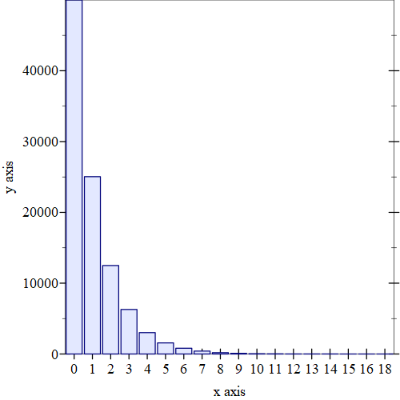
\includegraphics[width=10cm]{images/3.5.png}
    \caption{
        Histogram of geometric experiment: the \textit{x-axis} represents the values generated during the sampling phase; 
        the \textit{y-axis} represents the number of samples which have a specific value.
    }
    \label{fig:3-5}
\end{figure}


\subsection*{Exercise 3.7}
Convert Table~\ref{tab:es3-7} to a compact Racket program.
\begin{table}[H]
    \begin{center}
        \begin{tabular}{ccc}
            \hline
            A & B & P(A, B) \\
            \hline
            F & F & 0.14 \\
            F & T & 0.06 \\
            T & F & 0.4 \\
            T & T & 0.4 \\
            \hline
        \end{tabular}
    \end{center}
    \caption{Probabilities to be computed with a Racket program}
    \label{tab:es3-7}
\end{table}

\noindent Hint: fix the probability of A and then define the probability of B to depend on whether A is true or not. 
Run your Church program and build a histogram to check that you get the correct distribution.

\begin{lstlisting}
(define a ...)
(define b ...)
(list a b)
\end{lstlisting}

\paragraph{Solution}
The \texttt{a-b-model} has been defined as follows:
\begin{lstlisting}[caption={Model to compute the probabilities of A and B}, captionpos=b]
(define (a-b-model)
  (define a
    (flip 0.8))
  (define b
    (if a
        (flip 0.5)
        (flip 0.3)))
  (list a b))
\end{lstlisting}
The model does not contain the \texttt{rejection-sampler} because we do not need to compute a conditional probability.
The \texttt{a-b-model} defines first the variable \texttt{a} which has probability $0.8$ to be \textit{true}:
this probability can be computed by adding the last two rows of the Table~\ref{tab:es3-7}, indeed, the value of \texttt{A} in
the first two rows is \textit{false}, while in the last two is \textit{true}.
Then the probability of the variable \texttt{b} depends on the value of the variable \texttt{a}, indeed, if \texttt{A} is 
\textit{false}, then the probability that \texttt{B} is \textit{true} $ \frac{0.06}{0.06 + 0.14} = 0.3 $; while if
\texttt{A} is \textit{true}, then la probability that \texttt{B} is true is $ 0.5 $.

\begin{figure}[h]
    \centering
    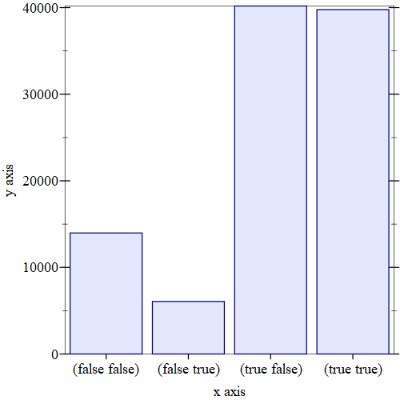
\includegraphics[width=10cm]{images/3.7.png}
    \caption{
        Histogram of A-B experiment: the \textit{x-axis} represents the values generated during the sampling phase; 
        the \textit{y-axis} represents the number of samples which have a specific value.
    }
    \label{fig:3-7}
\end{figure}

The experiment consists of generating $100000$ samples, the histogram of generated samples is shown in Figure~\ref{fig:3-7}.
It is possible to observe that the samples are distributed as the probability distribution defined in Table~\ref{tab:es3-7},
indeed, the number of samples with value false both for the variable \texttt{A} and \texttt{B} is about $14000$; the number of
samples with \texttt{A} \textit{true} is about $6000$ and the number of samples with value \textit{(true, false)} and 
\textit{(true, true)} is about $40000$ each. 
The number of samples is not exact because we are approximating the probability distribution by sampling.